\documentclass{article}

\usepackage{mathtools,amsfonts}
\usepackage{enumerate}
\usepackage{fullpage}
\usepackage{fancyvrb}
\usepackage{hyperref}


\begin{document}
\thispagestyle{empty}

\begin{center}
  \textbf{\Large Intermediate February Monthly Assignment Solutions}
\end{center}

\vspace{12pt}

\begin{enumerate}[1.]

\vspace{6pt}
\item % Jon
{\itshape The natural number $n$ can be replaced by $ab$ if $a + b = n$, where $a$ and $b$ are natural numbers. Can the number $2021$ be obtained from $22$ after a sequence of such
replacements?}

Suppose that the natural number $n$ can be obtained. Then since $(n - 1) + 1 = n$, we have that $(n - 1) \times 1 = n - 1$ can also be obtained. It follows that if we can obtain any number larger than $2021$ after a sequence of such moves, then we can also obtain $2021$ after a sequence of such moves.

Now note that $22 = 11 + 11$, so we can replace $22$ with $11 \times 11 = 121$. Then $121 = 100 + 21$, so we can replace $121$ with $100 \times 21 = 2100$. This is larger than $2021$, so we repeatedly replace the current number that we have with its predecessor until we obtain $2021$.


\vspace{6pt}
\item % DB-2014-1
{\itshape Prove that among the first $30000$ positive integers there are at least $22000$ composite numbers.}

Among the first $30000$ positive integers, there are $\frac{30000}{2} = 15000$ multiples of $2$, $10000$ multiples of $3$, and $6000$ multiples of $5$. There are then at most $15000 + 10000 + 6000 = 31000$ multiples of $2$, $3$, or $5$. But this counts each multiples of $6$, $10$, and $15$ twice, so we subtract the $5000 + 3000 + 2000 = 10000$ multiples of $6$, $10$, or $15$ to arrive at at least $31000 - 10000 = 21000$ multiples of $2$, $3$, or $5$. But now we have added each multiple of $30$ twice, but subtracted them $3$ times, so we add $\frac{30000}{30} = 1000$ to account for the multiples of $30$.

We thus see that among the first $30000$ positive integers, there are $22000$ that are a multiple of $2$, $3$, or $5$. These are all composite except for $2$, $3$, or $5$ themselves, so we need only find $3$ more composite numbers below $30000$ that are not divisible by any of these. The numbers $49$, $77$, and $121$ will do.


\vspace{6pt}
\item % Salvador 2017 9th grade Q2
{\itshape Let $a$ and $b$ be positive real numbers such that $2a^2 +2b^2 = 5ab$.
If $|x|$ denotes the absolute value of $x$, calculate
\[ \left|\frac{a+b}{a-b}\right|. \]}

We rewrite the given equation as
\[
	(a + b)^2 + (a - b)^2 = \frac{5}{4} \left( (a + b)^2 - (a - b)^2 \right)	
\]
we can be rearranged to become
\[
	\frac{1}{4} (a + b)^2 = \frac{9}{4} (a - b)^2	
\]
or
\[
	\left( \frac{a + b}{a - b} \right)^2 = 9.
\]
By taking square-roots, it follows that
\[
	\left| \frac{a + b}{a - b} \right| = 3.	
\]



\vspace{6pt}
\item % Taariq, stolen from AOPS
{\itshape Triangle $ABC$ is a right angled triangle with $\angle C = 90^{\circ}$. $P$ is placed randomly inside $\triangle ABC$. What is the probability that the area of $\triangle PBC$ is less than half of the area of $\triangle ABC$?}

\begin{figure}[!ht]
	\centering
	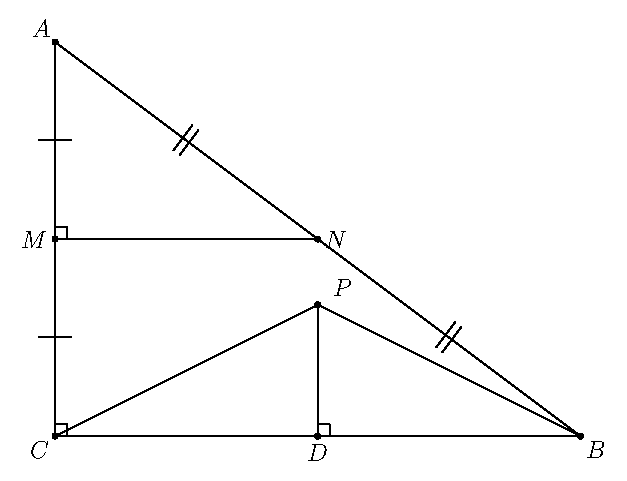
\includegraphics{intermediate_february_problem4.eps}
	\caption{Problem 3}
\end{figure}

Let the foot of the perpendicular from $P$ onto $BC$ be $D$. Let $M$ and $N$ be the midpoints of $AC$ and $BC$ respectively. We note that the area of $PBC$ is given by $\frac{1}{2} BC \times PD$, and that the area of triangle $ABC$ is given by $\frac{1}{2} BC \times AC$.

It follows that the area of triangle $PBC$ is less than half of that of $ABC$ if and only if $PD < \frac{1}{2} AC$. We see that this is equivalent to $P$ not lying in the triangle $AMN$. Now the area of triangle $AMN$ is given by
\[
	\frac{1}{2} MN \times AM = \frac{1}{2} \left(\frac{1}{2} BC \right) \times \left(\frac{1}{2} AC\right) = \frac{1}{4} |ABC|	
\]
where $|ABC|$ denotes the area of triangle $ABC$. It follows that the probability that a randomly chosen point chosen inside triangle $ABC$ lies in $AMN$ is
\[
	\frac{|AMN|}{|ABC|} = \frac{1}{4},	
\]
and so the probability that $P$ \emph{does not} lie in triangle $AMN$ is $1 - \frac{1}{4} = \frac{3}{4}$.


\vspace{6pt}
\item % Danielle/Taariq
{\itshape Let $c$ and $d$ be positive divisors of a natural number $n$ such that $c > d$. Prove that $$c > d + \frac{d^2}{n}.$$}

Let $n = kc = md$. The inequality that we want to prove is then equivalent to
\[
	\frac{n}{k} > \frac{n}{m} + \frac{\frac{n^2}{m^2}}{n} \iff \frac{1}{k} > \frac{1}{m} + \frac{1}{m^2} \iff m^2 > mk + k.
\]
Since $c > d$, we have that $k < m$, and so $k \leq m - 1$, and so we have that
\[
	mk + k = k(m + 1) \leq (m - 1)(m + 1) = m^2 - 1 < m^2
\]
which proves the desired result.


\vspace{6pt}
\item % Ireland 2018 Q9
{\itshape Suppose $a,b,c > 0$ and $\sqrt{a-b} +\sqrt{a-c} > \sqrt{b+c}$. Prove that $a > \dfrac{3}{4} (b+c)$.}

Suppose that $a \leq \dfrac{3}{4} (b + c)$. We will show that $\sqrt{a-b} +\sqrt{a-c} \leq \sqrt{b+c}$. Since $a \leq \dfrac{3}{4} (b + c)$, we have that
\[
	\sqrt{a-b} +\sqrt{a-c} \leq \sqrt{\frac{3}{4}(b + c) - b} + \sqrt{\frac{3}{4}(b + c) - c} = \frac{1}{2} \left(\sqrt{3c - b} + \sqrt{3b - c}\right).
\]

We thus wish to show that
\[
	\dfrac{1}{2} \left(\sqrt{3c - b} + \sqrt{3b - c}\right)  \leq \sqrt{b + c}.
\]
By squaring both sides, this is equivalent to
\[
	(3c - b) + (3b - c) + 2\sqrt{(3c - b)(3b - c)}  \leq 4(b + c).
\]
We move the terms not under the square-root to the right hand side, divide by $2$, and square again to obtain
\[
	(3c - b)(3b - c) \leq (b + c)^2.
\]
Expanding each side of this inequality leads us to want to prove that
\[
	10bc - 3b^2 - 3c^2 \leq b^2 + 2bc + c^2
\]
which is equivalent to
\[
	4(b - c)^2 \geq 0
\]
and so we are done.


\end{enumerate}

\end{document}
